As detailed by \citet{limpens2023pathway}, the analysis carried out in this work can be applied to any regional whole-energy system. As a densely-populated and highly-industrialised country with limited local renewable potentials (mainly solar and wind), the transition of Belgium from a fossil-dominated system in 2020 (Appendix \ref{app:bel_2020}) to carbon-neutrality in 2050 makes it an intricate case study. Moreover, this case study and the subsequent analyses can be transferred - to some extent - to other industrialised countries highly dependent on fossil fuels with limited local renewable potentials (\eg the Netherlands or Germany) \cite{dommisse2020modelling}. This section presents the different demands to satisfy as well as the resources available and the conversion technologies to supply those. The focus here is given to the renewable molecules to import from abroad as well as the techno-economic details of \gls{SMR}. For a comprehensive understanding and detailed descriptions of the technologies, please refer to the documentation \cite{readthedocs_pathway}. Finally, the \ce{CO2}-budget over the 2020-2050 transition is presented.


\section{Demands}
\label{sec:cs:demand}

End-use demands, exogenously imposed as inputs to the model, are characterised by yearly quantities to satisfy and are also distributed over the different hours of each representative years of the transition, in order to account for their daily or seasonal variability. In this work, the yearly end-use demands (EUD) for all sectors are calculated from the rather slightly increasing forecast proposed by the European Commission for Belgium (Appendix 2 in report \cite{EuropeanCommission2021}). Although, given a significant and unsubstantiated discrepancy in the non-energy use forecasts compared to their previous report (\ie +80\% over the 2020-2030 time window), the evolution trend of the \gls{NED} of the current work has been inferred from the previous edition, published in 2016, \cite{EuropeanCommission2016}. Looking at \Cref{fig:cs_demands}, between 2020 and 2050, one observes a noteworthy increase of the electricity (+40\%), passenger (+45\%) and freight mobility (+35\%) demands. The rise of the non-energy demand is more limited, \ie +6\%, whereas the heating demands is forecast to decrease: -11\% and -3\% respectively for the low and high-temperature heat demands. Regarding the center graph of \Cref{fig:cs_demands}, it is the aggregation of the same data as in the left graph but per category, rather than per sector, with the non-energy demand being associated with the industry. This illustrates how industrialised is Belgium, compared to households and services, and, consequently, highly energy-intensive. The right graph of \Cref{fig:cs_demands} gives the passenger and the freight mobility. The sharp increase from 2020 to 2025 is due the COVID-crisis that has significantly reduced these demands in 2020. As far as the hourly discretisation of these demands is concerned, time series are based on historical values of 2015 for parts of electricity and low-temperature heating demands \cite{Limpens2020}. A daily time series is used for the passenger mobility and applied similarly to every typical days. Finally, for the other demands, the yearly demand is distributed uniformly over the different hours of the year.

\begin{figure}[htbp!]
\centering
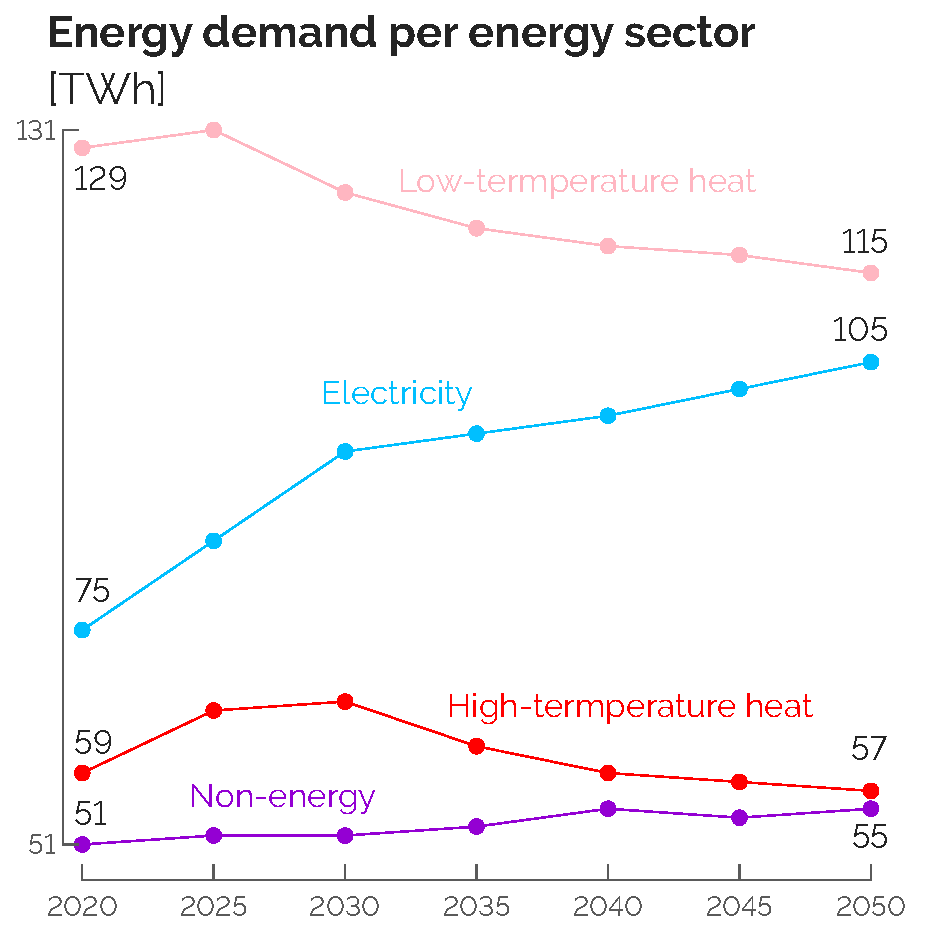
\includegraphics[width=0.32\textwidth]{EUD_sec.pdf}
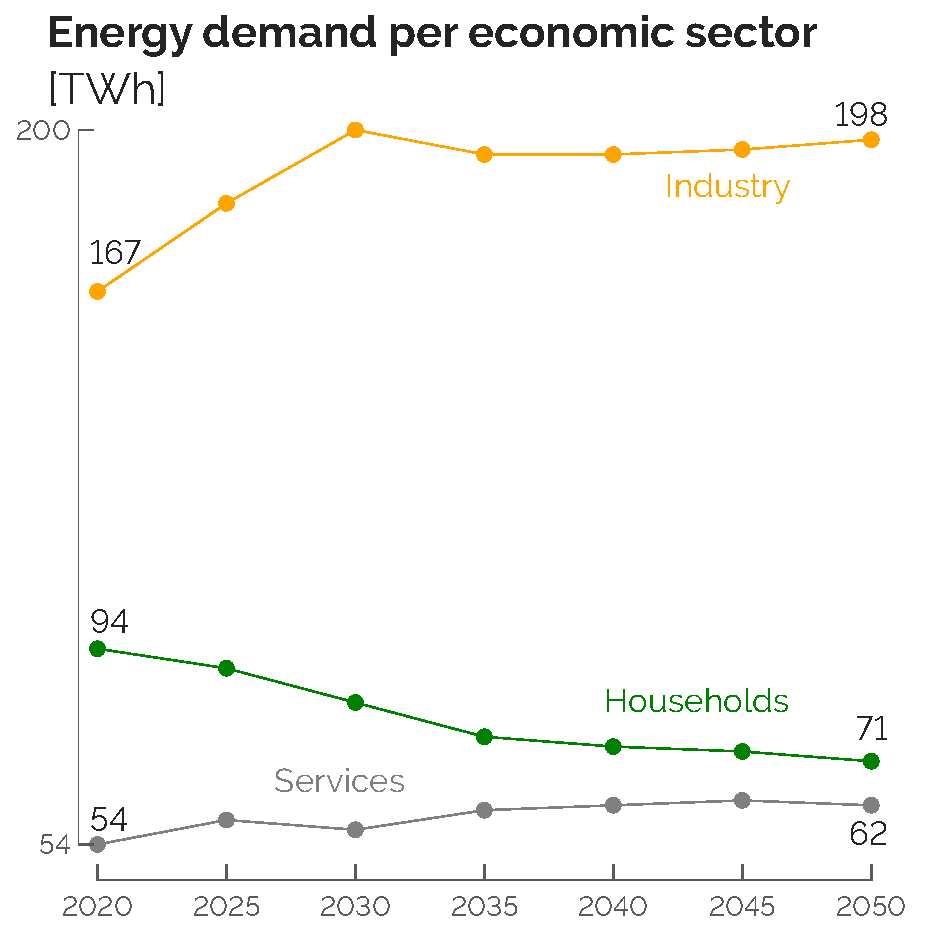
\includegraphics[width=0.32\textwidth]{EUD_cat.pdf}
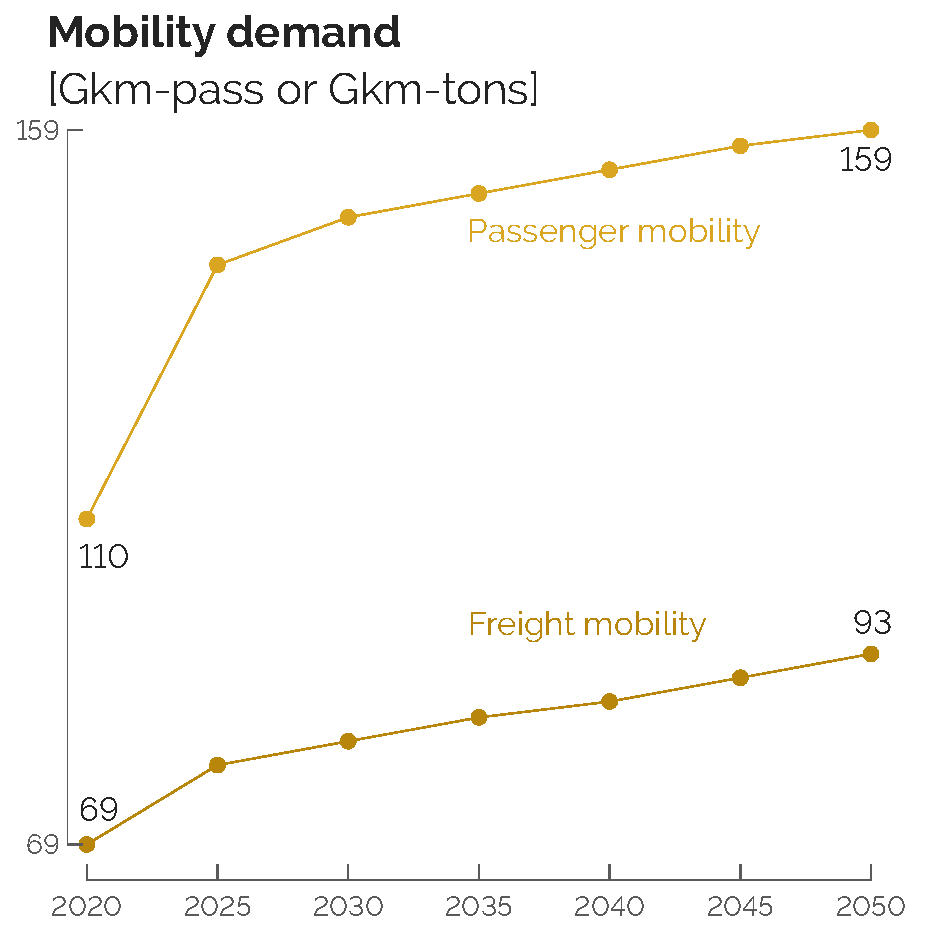
\includegraphics[width=0.32\textwidth]{EUD_mob.pdf}
\caption{EnergyScope splits the whole-energy system end-use demands (EUD) into two sets: (non)-energy and transport-related. This figure presents the nominal values of each of these demands. In the center graph, the non-energy demand has been fully associated with the industrial demand. As detailed by \citet{rixhon2022integration}, the non-energy demand is expressed in tons of physical products (\ie \glsxtrfull{HVC}, ammonia and methanol) and then translated into their respective energy equivalent, in TWh. Graphs have been adapted from \cite{limpens2023pathway}.}
\label{fig:cs_demands}
\end{figure}


\section{Resources}
\label{sec:cs:resources}
To supply the aforementioned demands, EnergyScope Pathway implements a variety of resources defined by their cost of purchasing, $\mathit{c}_{\mathrm{op}}$, their global warming potential, $\mathit{gwp}_{\mathrm{op}}$, as well as their 
availability, as detailed by \citet{limpens2023pathway}. \Cref{fig:cs_resources_cost} depicts the evolution the respective costs of purchasing. Regarding ``renewable electrofuels'', these are in line with the recent study of \citet{genge2023supply} who carried out an extensive review and ``meta-analysis\cite{grant2009typology,page2021prisma} of 30 studies on the supply costs of chemical energy carriers''. Then, besides their cost, the resources are either limited or unlimited in terms of availability and either renewable or not. The limitation in terms of availability can be direct or indirect. On the one hand, woody (23.4\,TWh) and wet biomass (38.9\,TWh) are limited by their local potentials and the consumption of waste (17.8\,TWh) and coal (33.4\,TWh) is assumed not to exceed the current use. On the other hand, wind, solar, hydro and uranium are limited by the technical potentials respectively, of \gls{PV} panels (59.2\,GW), onshore (10\,GW) and offshore (6\,GW) wind turbines, run-of-the-river power plants (0.1\,GW) and nuclear power plants (6\,GW). As \gls{SMR} are foreseen, if installed, to be around the same locations (\ie Thiange and Doel) as the conventional nuclear power plants and using the same area in kW/ha, the same 6\,GW are assumed to be the maximum capacity for \gls{SMR}. This is even without considering the potential limit due to the local availability, in terms of volume and flow rate, of enough water that would be a more socially-accepted solution than cooling towers exhausting a dense plume. Imported electricity is limited in two ways: the potential of instantaneous capacity of interconnection with neighbouring countries (\ie 11.9\,GW by 2050 \cite{ELIA_2050}) and a limitation to 30\% of the yearly electricity end-use demand (\ie 32.4\,TWh by 2050). In the current work, the electrofuels (\ie e-methane, e-hydrogen, e-methanol and e-ammonia) are assumed to be ``sustainable" in the sense that they do not increase the concentration of \ce{CO2} in the atmosphere \cite{rixhon2021terminology}. In practice, it means that their \gls{GWP} is assumed to be zero in the model. Regarding specifically these electrofuels, the \citet{h2coalition} has carried out an extensive techno-economic analysis to estimate their respective cost of purchasing, after having identified some key locations from which importing these energy carriers (\eg Chile, Australia or Morocco). As the amount to import from each of these locations is hard to forecast, the current work considers the average cost between the different locations. Besides these, every other resource has its specific \gls{GWP} like coal ($\mathit{gwp}_{\mathrm{op,coal}}=0.40$\,kt$_{\ce{CO2},\text{eq}}$/GWh), natural gas ($\mathit{gwp}_{\mathrm{op,NG}}=0.27$\,kt$_{\ce{CO2},\text{eq}}$/GWh) or the fossil-based molecules equivalent to the electrofuels (\eg $\mathit{gwp}_{\mathrm{op,ammonia}}=0.46$\,kt$_{\ce{CO2},\text{eq}}$/GWh or $\mathit{gwp}_{\mathrm{op,methanol}}=0.41$\,kt$_{\ce{CO2},\text{eq}}$/GWh).

\begin{figure}[htbp!]
\centering

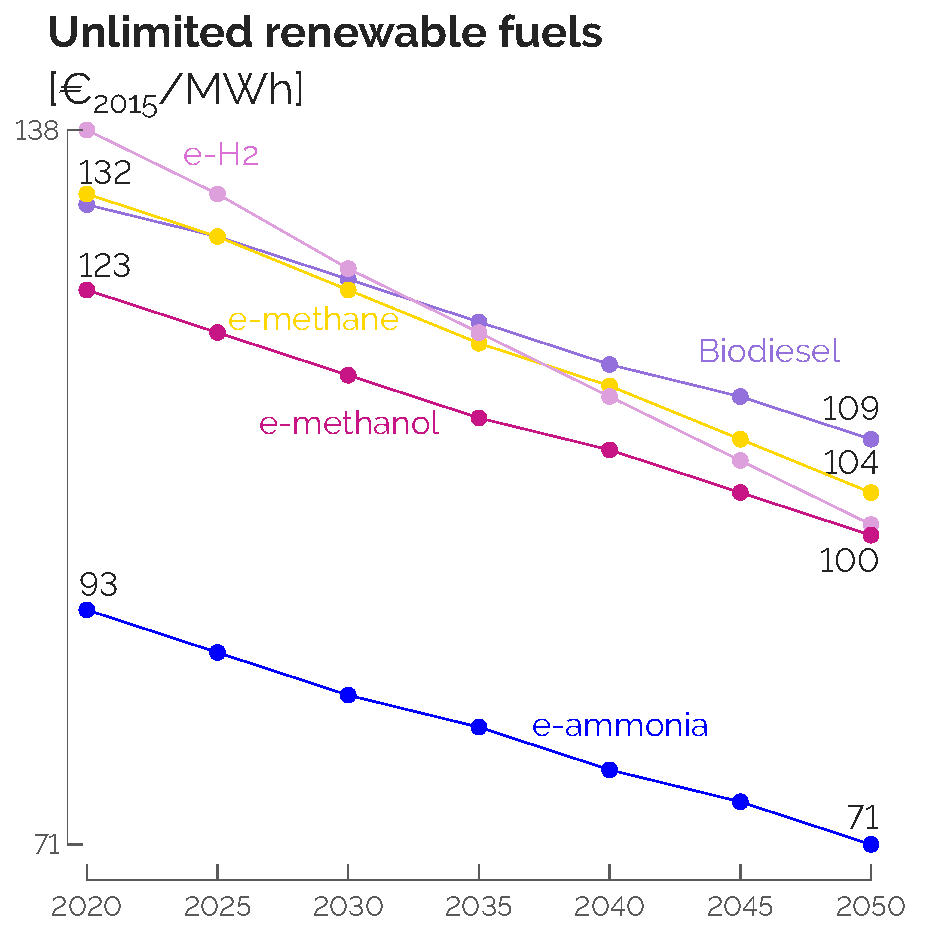
\includegraphics[width=0.32\textwidth]{Res_ren.pdf}
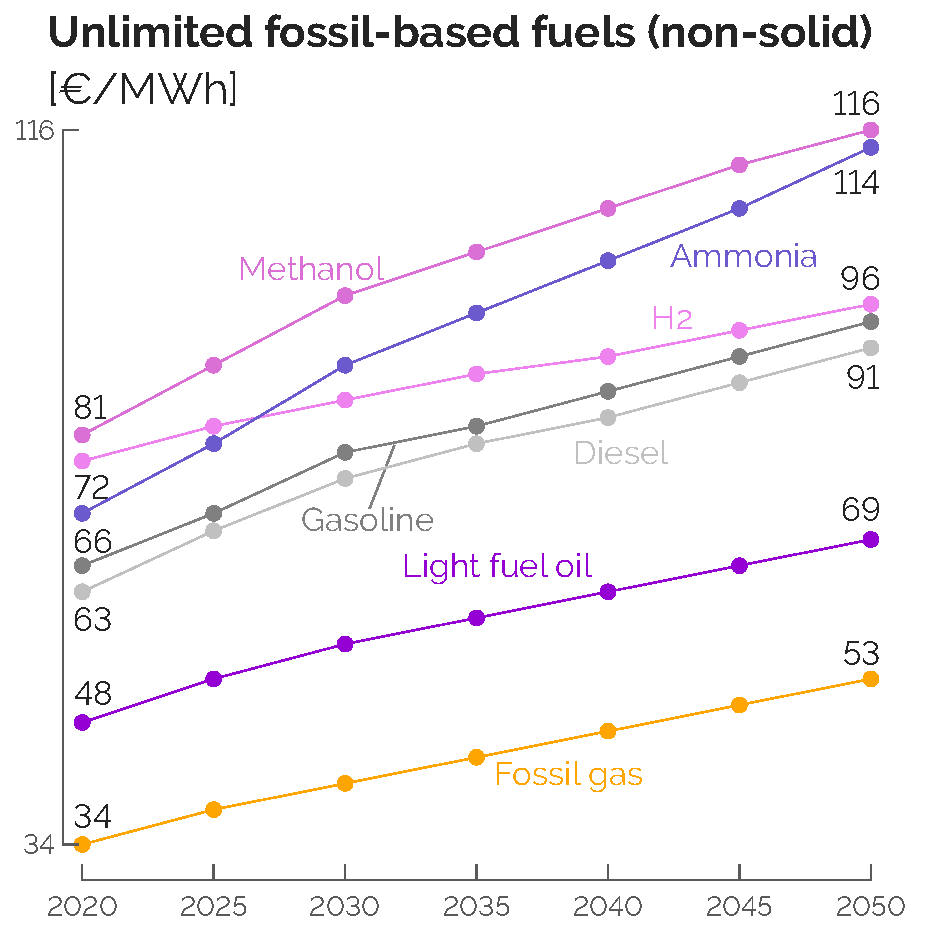
\includegraphics[width=0.32\textwidth]{Res_foss.pdf}
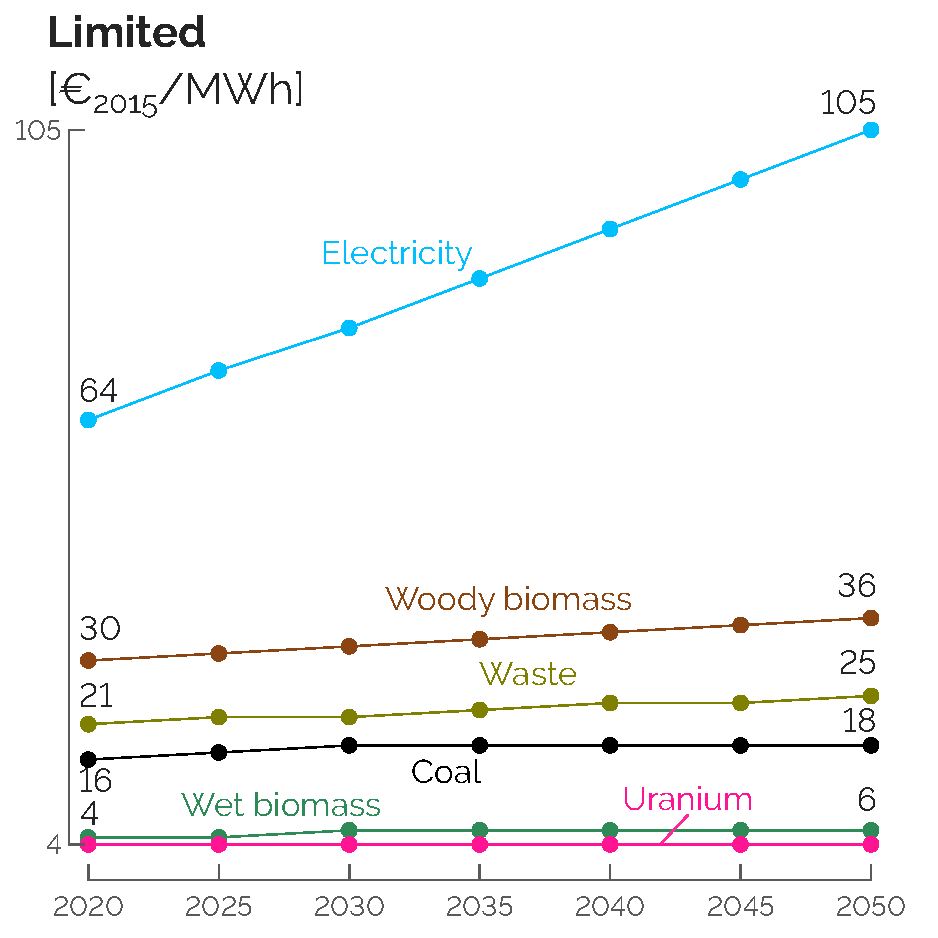
\includegraphics[width=0.32\textwidth]{Res_others.pdf}
\caption{Cost of purchasing the different resources. Besides the free local renewables (\ie sun, wind and hydro) limited by technical potentials, EnergyScope accounts for renewable energy carriers and their respective fossil counterparts (left and center graphs). These fuels can be imported from abroad without limitation on their availability. Other carriers are limited either by their local potentials (\ie biomass and waste) or other considerations like the power grid interconnections or the capacity of nuclear power plants.}
\label{fig:cs_resources_cost}
\end{figure}


\section{SMR and other conversion technologies}
\label{sec:cs:technologies}
Finally, as the end-use demands are defined as energy (and non-energy with the \gls{NED}) services rather than a certain quantity of oil or solar irradiance, technologies are implemented to convert these resources into the end-use demands. Besides their CAPEX, OPEX and lifetime defined in Section \ref{subsec:meth:ES_Pathway}, production and conversion technologies (\ie \gls{CCGT}, car or boiler) have a conversion efficiency whereas storage technologies (\ie thermal storage, battery or molecule storage) exhibit their own charge/discharge losses. Eventually, there are also infrastructure technologies like the grid or the \gls{DHN} that allow to account for the investment necessary, respectively, to integrate more intermittent renewables in the power sector and the expand the use of centralised heating systems.

A specific attention is to put on the implementation of \glsxtrfull{SMR} whereas the 6\,GW of conventional nuclear are assumed to drop to 2\,GW in 2025 and total phase-out by 2035. Similarly to the analysis of \citet{PATHS2050}, a Belgian consortium for energy research, and in line with the Belgian Nuclear Research Centre (SCK-CEN) \cite{SCK-CEN_SMR}, \gls{SMR} are implemented with the features listed in \Cref{tab:SMR_features}. Where most of the features are similar to conventional nuclear power plants, it differs from these on two main points: their potential year start, 2040, and their flexibility. Indeed, unlike the current nuclear power plants, constrained in the model to produce a constant power output at every hour of the year (\ie baseload production as it is actually the case in Belgium), SMRs, are flexible in the sense that their production can vary between 0 and their full capacity independently at any hour of each representative year. Here, the authors simplify SMRs as only producing electricity and assume that the after-heat is lost to the atmosphere anyway.


\begin{table}[htbp!]
\caption{Nominal features of the SMRs in EnergyScope. \gls{SMR} exhibits the advantage to have a fully flexible production (\ie between 0 to the full capacity) unlike conventional nuclear that is constrained to produce a constant baseload at every hour of the year. $^{(a)}$ This annual availability accounts for yearly maintenance where the reactors might not operate or, at least, not at their maximum capacity. $^{(b)}$ 2040 is the soonest year at which \gls{SMR} could be available, optimistically assuming industrial prototypes being completed by 2035 and 5 additional years for their commercial installation.}
\label{tab:SMR_features}
\centering
\begin{tabular}{l c c|c}
\toprule
\multirow{2}{*}{\textbf{Feature}} & \multirow{2}{*}{\textbf{Value}} & \multirow{2}{*}{\textbf{Unit}} & \textbf{Similarity with}\\
 & & & \textbf{conventional nuclear}\\
\midrule
CAPEX & 4850 & €/kW & \checkmark\\
Annual OPEX & 103 & €/kW/year & \checkmark\\
Lifetime & 60 & year & \checkmark\\
Efficiency & 40\% & -& \checkmark\\
Maximum capacity & 6 & GW & \checkmark\\
Annual availability & 85\%$^{(a)}$ & -& \checkmark\\
\midrule
Operational year & 2040$^{(b)}$ & - & \xmark\\
Flexibility & Full & - & \xmark\\
\bottomrule							

\end{tabular}
\end{table}

For the sake of comparison, \Cref{fig:LCOE} gives the \gls{LCOE} of the principal technologies to produce electricity, based on the computation used by \citet{limpens2021generating}. Compared to the other flexible generation units, \gls{SMR} is significantly more cost-effective. In addition, we see that \gls{CCGT} supplied by e-ammonia outcompetes its e-methane equivalent, unlike their respective fossil-based equivalent.

\begin{figure}[htbp!]
\centering
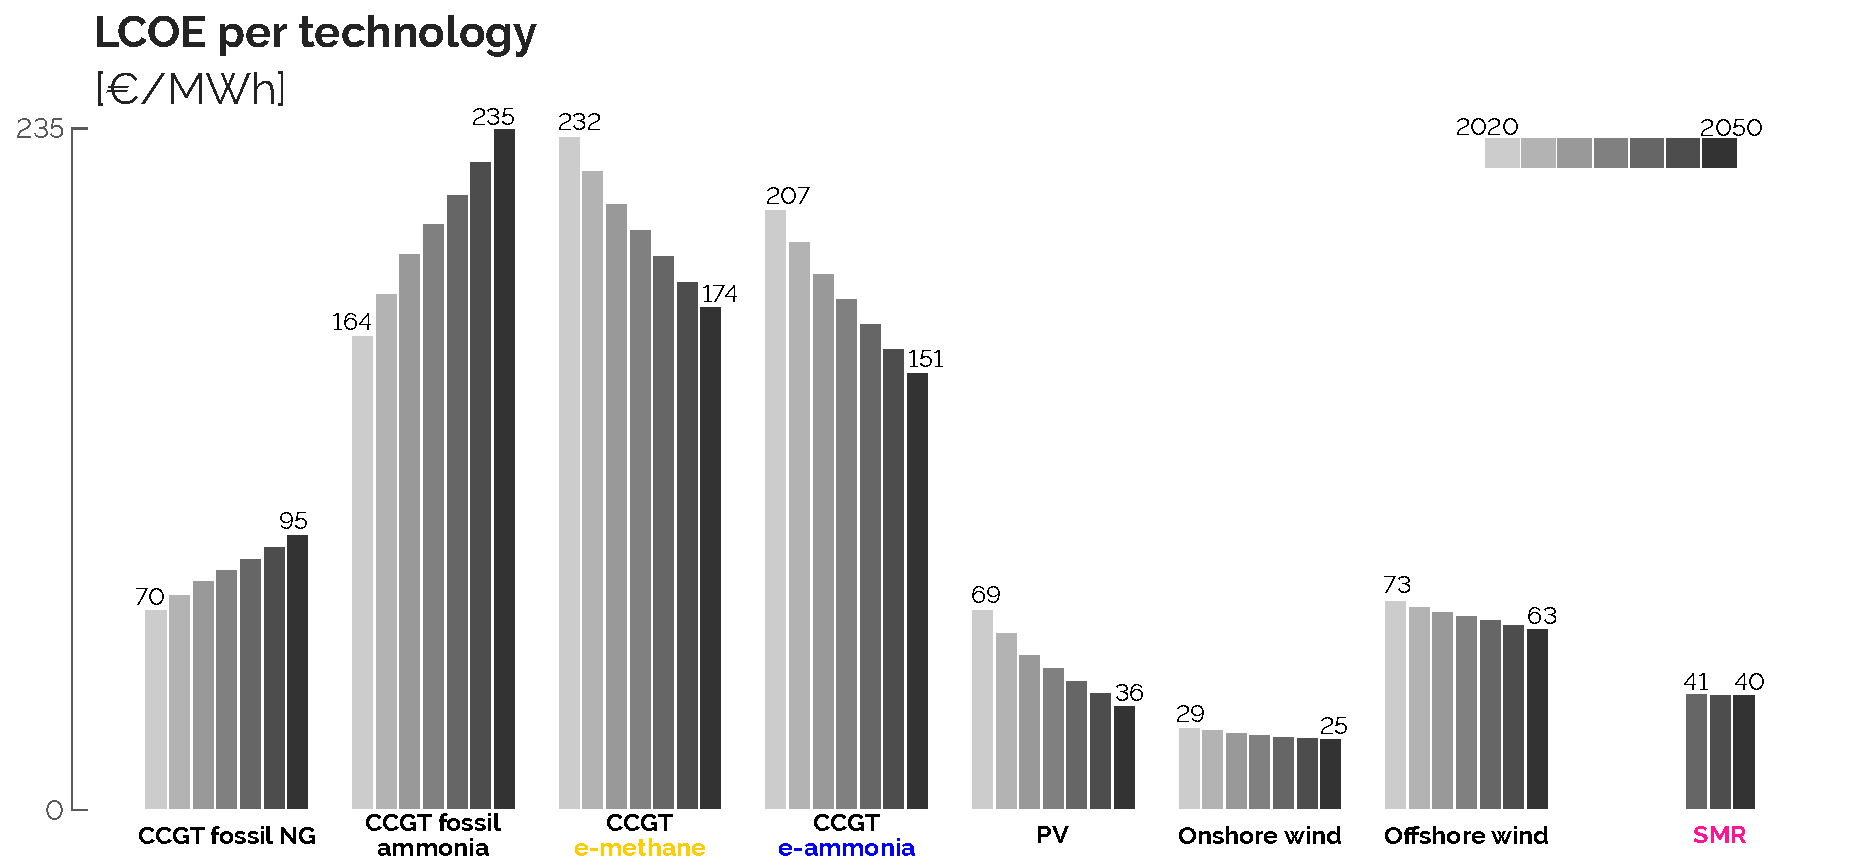
\includegraphics[width=0.6\textwidth]{LCOE.pdf}
\caption{Levelised cost of energy (LCOE) for the main technologies in the power sector. Where \gls{SMR} is cheaper than the other flexible options, CCGT running on e-ammonia is, a priori, cheaper than its e-methane alternative.}
\label{fig:LCOE}
\end{figure}

\section{\ce{CO2}-budget for the transition}
\label{sec:cs:CO2-budget}
In most of the studies carried out on the pathway optimisation of a whole-energy system, a \ce{CO2}-trajectory is \textit{a priori} set to reach carbon-neutrality by 2050. \citet{nerini2017myopic} used the emission trajectory indicated by the UK's Committee on Climate Change in their analysis of the impact of limited foresight to achieve the target of 80\% reduction of \gls{GHG} by 2050 in the United Kingdom. In their assessment of the impacts of economy-wide emissions policies in the water-energy-land nexus, \citet{licandeo2023assessing} analysed different \ce{CO2}-trajectories considering more or less severe water scarcity for the US. \citet{poncelet2016myopic} with LUSYM (Leuven University SYstem Model) and \citet{PATHS2050} with TIMES-BE also set decreasing emission trajectories in their analysis of respectively the Belgian power sector and whole-energy system.  Others only set the objective as the carbon-neutrality by 2050. For instance, \citet{heuberger2018impact} investigated the impact of different factors (\eg limit of the foresight in the future, availability of ``unicorn technologies'' or committed versus market-driven decarbonisation strategies) to reach this ultimate objective in the UK system.

In this work, the effect of greenhouse gases is cumulative over time and a constraint is set on the overall emissions of the transition---a \ce{CO2}-budget for the transition. This budget (1.2\,Gt$_{\ce{CO2},\text{eq}}$) corresponds to the proportion of Belgium's emissions in the world emissions in 2020 (34.8\,Gt$_{\ce{CO2},\text{eq}}$ \cite{ourworldindata_CO2_world}) applied to the global budget to have a 66\% chance of limiting warming to 1.5°C of 420\,Gt$_{\ce{CO2},\text{eq}}$ \cite{IPCC_CO2_budget}. Therefore, in this work, a limit has been put on $\emph{gwp\textsubscript{lim,trans}}=1.2\,\text{Gt}_{\ce{CO2},\text{eq}}$ in
Eq.\,(\ref{eq:limit_gwp_trans}). This is another sign of the urgency to act to mitigate climate change as this 30-year budget represents only 10 years of the current emissions. Compared to a linear decrease from the current emissions, as done by \citet{limpens2023pathway}, this budget represents a 60\% reduction of the cumulative emissions over the transition.  Appendix \ref{app:CO2_budget} compares the emissions trajectory between the REF case and a case (without \gls{SMR}) where the linear decrease is imposed between 2020 and carbon-neutrality in 2050.

\textbf{GRANDFATHERING dans la vision d'attribuer le budget CO2 donné à la Belgique. Defining the share of the safe operating space from How to bring absolute sustainability into decision-making: An industry case study using a Planetary Boundary-based methodology. Sharing the safe operating space}